\ifja
    \chapter*{著者プロフィール}
    \addcontentsline{toc}{chapter}{著者プロフィール}
    \begin{center}
        \centering
        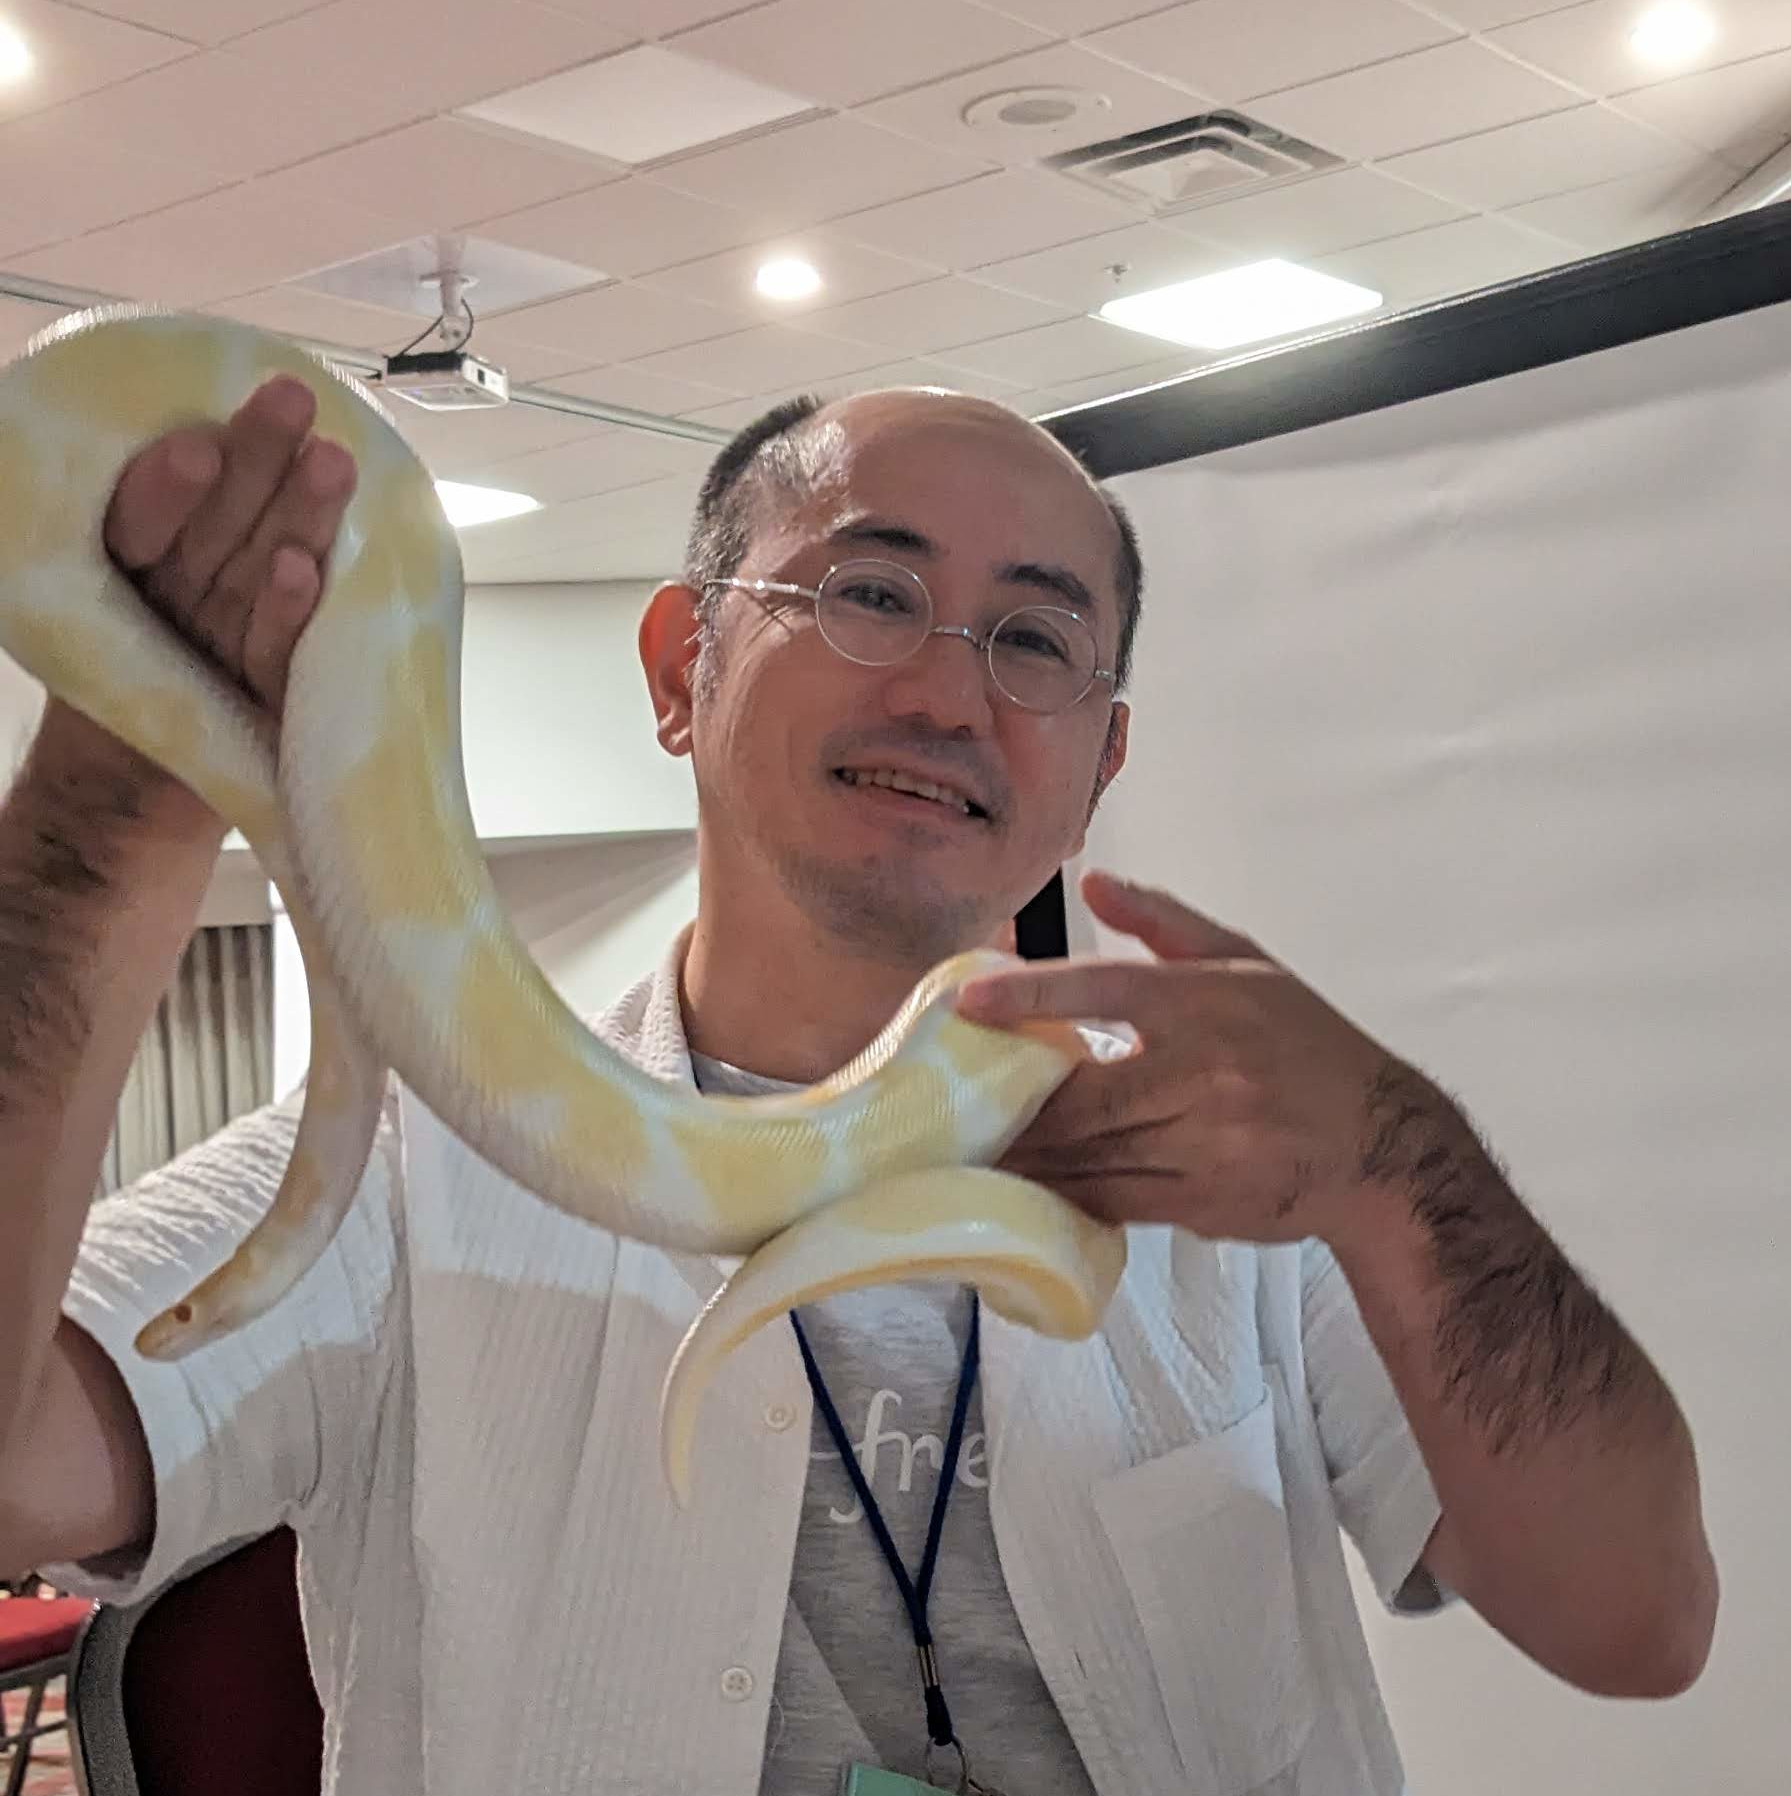
\includegraphics[width=0.4\linewidth, keepaspectratio]{src/images/author.jpg}
        \label{fig:author}
    \end{center}
    \textbf{Masahiro Sugaya}

    \exSNLP 創始者。

    ベイジアンハッカー。東京大学大学院理学系研究科物理学専攻修士課程修了。固定磁場強収束加速器（FFAG）のビーム物理および非線形位相空間制御の研究に従事。コンピューターエンジニアを経て、脳科学・ベイズ統計・情報幾何学・サイバネティクスを統合した決定論的認知科学アプローチ「 \exSNLP 」を体系化。

    米国Society of NLP\texttrademark 公認NLPトレーナー。Dr. Richard Bandlerの催眠指導のもと、世界各国をトランス状態で放浪・探求。インド・ヨガの聖地リシケシやチベット亡命政府の拠点ダラムシャラを巡礼し、チベット仏教の高僧ゲシェ・カルサン・ダムダル師より出家を許可されるも在家を選択。仏教徒ではなくサイエンティストの道を選んだ。さらに、長野の曹洞宗無量寺にて現代屈指の禅僧・青山俊董老師より禅の手ほどきを受け、坐禅による徹底した身心脱落を追究。あわせてS.N. ゴエンカ氏のヴィパッサナー瞑想10日間コースを数度修了し、アルボムッレ・スマナサーラ長老からも指導を受けるなど、チベット密教・曹洞禅・初期仏教（テーラワーダ）を横断し、身体感覚のスキャンとサティ（気づき）を通じた「内受容感覚の制御」および「自我（Ego）の脱同一化」を身体知として体得する。

    また、対人行動・非言語情報の精密分析において、ポール・エクマン（Paul Ekman）グループ認定「METT（Micro Expression Training Tool）Advanced」を修了・保有。加えて、リチャード・ボルスタッド（Richard Bolstad）開発の「Transforming Communication（TC）」認定資格を有する。

    理論物理学の数理的厳密性、東洋伝統思想・臨床催眠の変容技術、そして微表情分析の客観的プロファイリングを架橋し、現実の非エルゴードな動的環境をハックする独自の指導・研究を展開している。

\else
    \chapter*{Author Profile}
    \addcontentsline{toc}{chapter}{Author Profile}
    \begin{center}
        \centering
        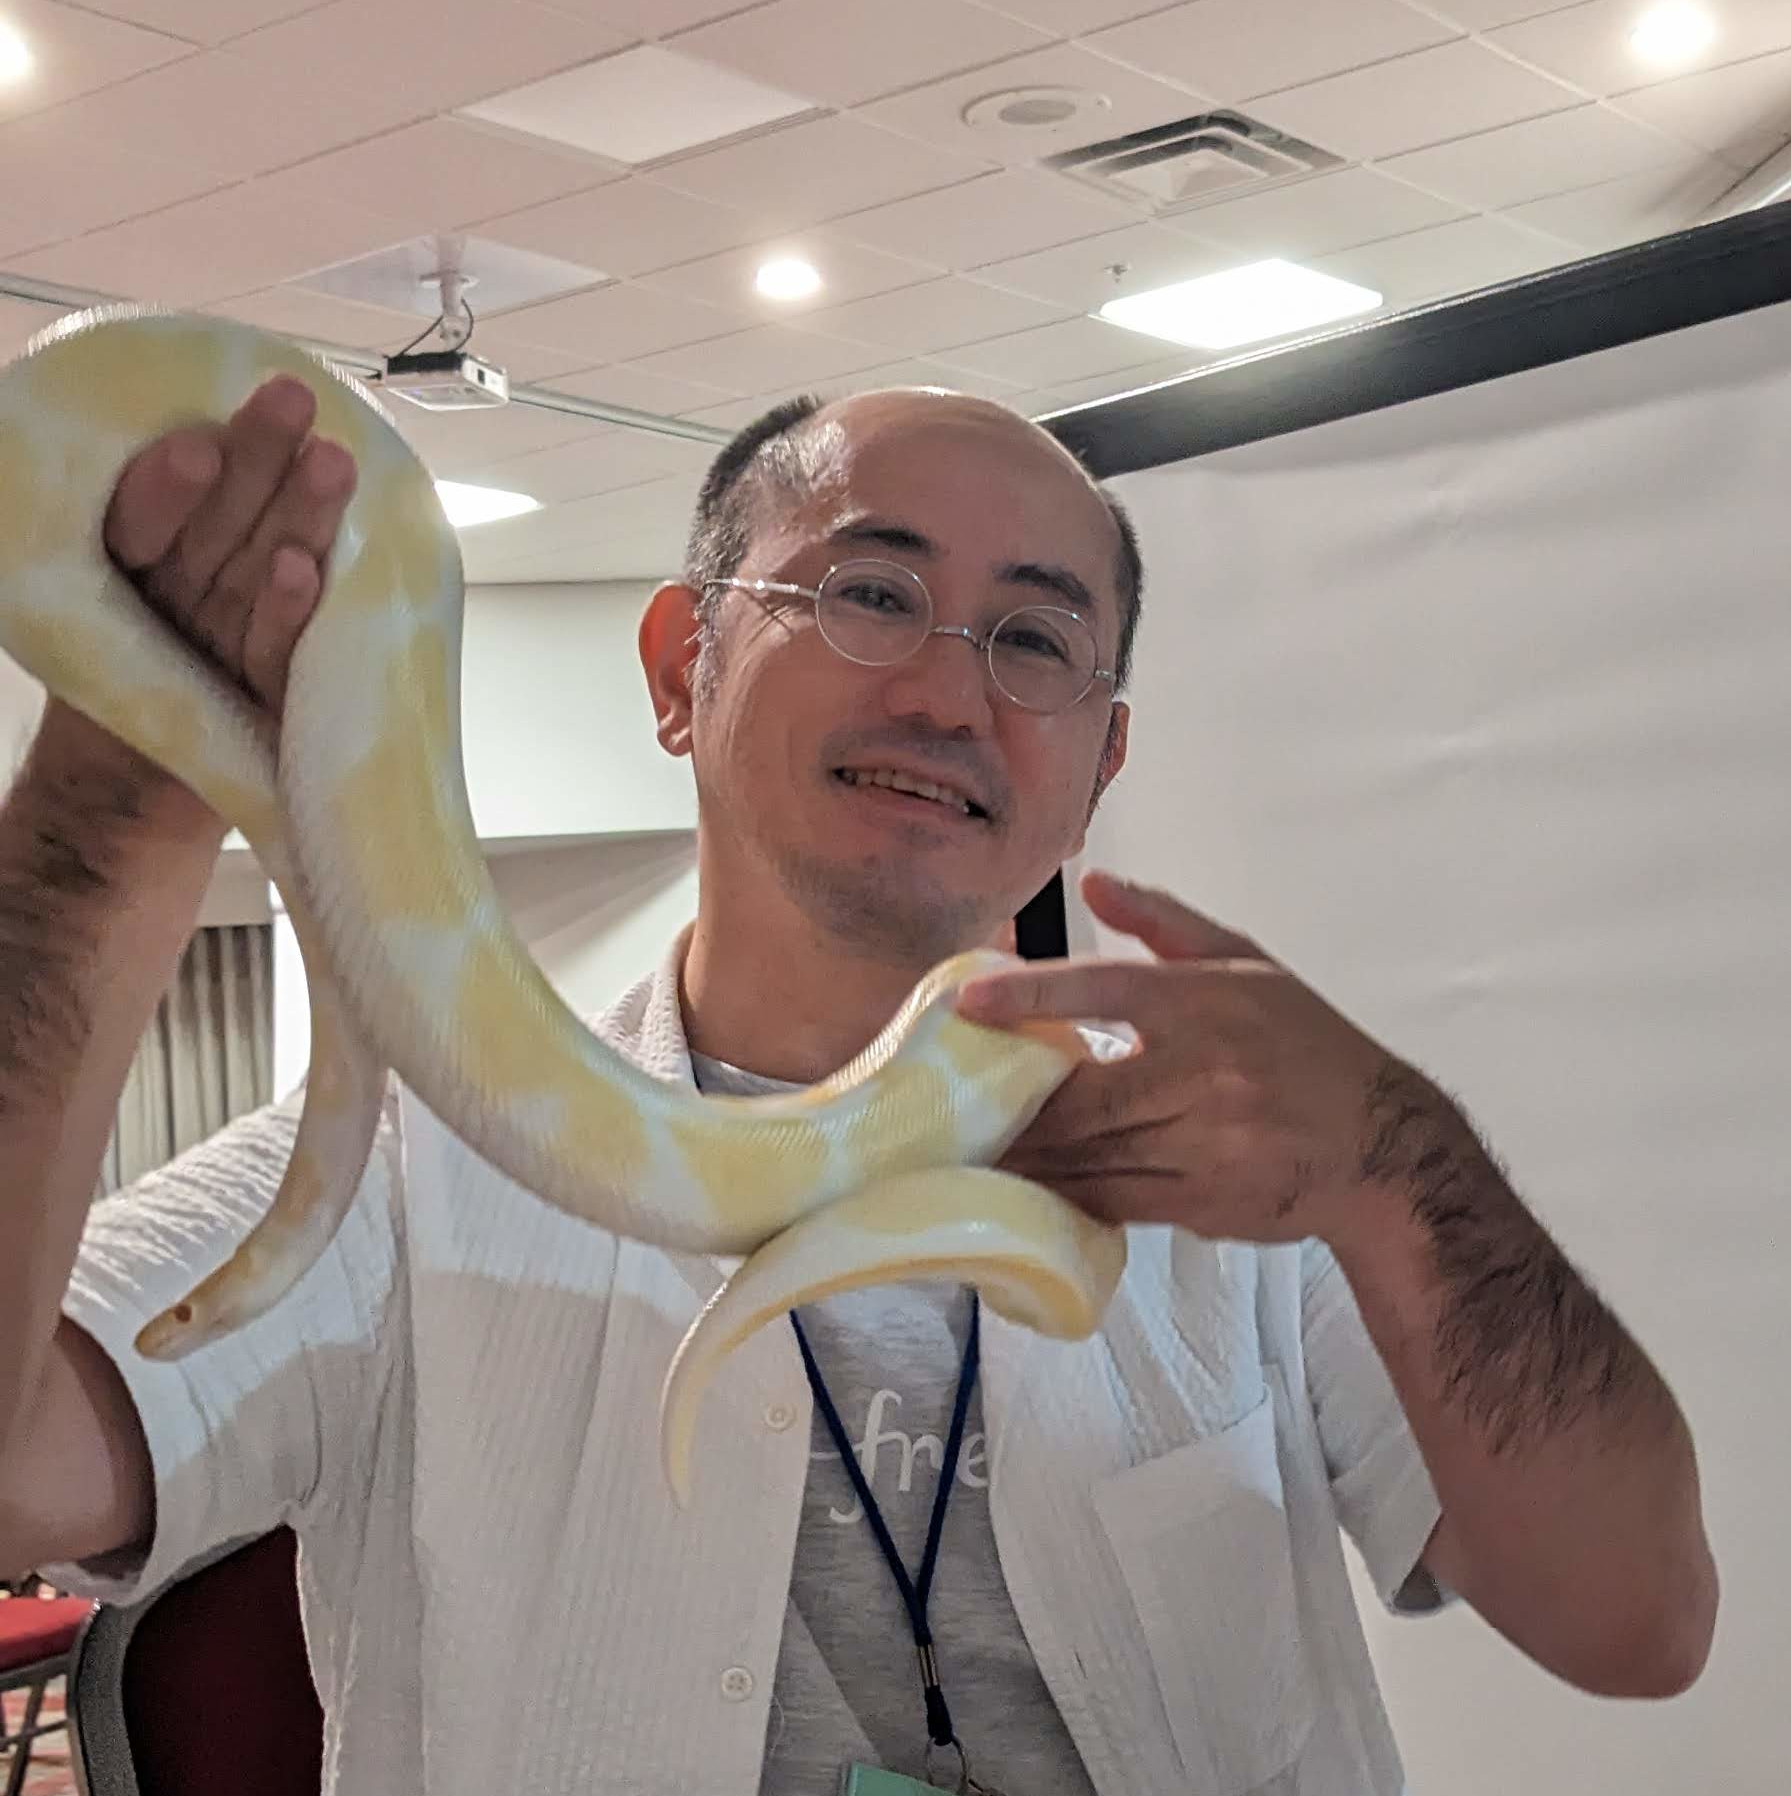
\includegraphics[width=0.4\linewidth, keepaspectratio]{src/images/author.jpg}
        \label{fig:author_en}
    \end{center}
    \textbf{Masahiro Sugaya}

    Founder of \exSNLP.

    Bayesian Hacker. M.Sc. in Physics from the Graduate School of Science, The University of Tokyo. Conducted research on beam physics and nonlinear phase space control in Fixed-Field Alternating Gradient (FFAG) accelerators. Following a career as a computer systems engineer, he formulated \exSNLP---a deterministic cognitive science framework integrating neuroscience, Bayesian inference, information geometry, and cybernetics.

    Licensed NLP Trainer certified by The Society of NLP\texttrademark. Under the direct hypnotic mentorship of Dr. Richard Bandler, he traversed the globe in exploratory trance states. His pilgrimages led him to Rishikesh, the cradle of Yoga, and Dharamshala, the seat of the Tibetan Government in Exile. Although granted formal monastic ordination permissions by the venerable Tibetan Buddhist master Geshe Kelsang Damdul, he chose to remain a lay practitioner---choosing the path of an empirical scientist rather than that of a religionist. Furthermore, he studied Soto Zen under Roshi Shunto Aoyama, one of Japan's preeminent contemporary Zen masters at Muryo-ji Temple in Nagano, pursuing the radical casting off of body and mind (\textit{shinjin datsuraku}). Having completed multiple 10-day Vipassana meditation retreats in the tradition of S.N. Goenka and received personal instruction from the Theravada Elder Ven. Alubomulle Sumanasara, he cross-disciplinary unified Tibetan Tantra, Soto Zen, and Early Theravada traditions, mastering interoceptive calibration and ego-disidentification as somatic architecture through body scanning and \textit{sati} (mindfulness).

    In interpersonal behavioral and nonverbal profiling, he completed and holds advanced credentials in the Paul Ekman Group's Micro Expression Training Tool (METT Advanced). Additionally, he is a certified practitioner in Transforming Communication (TC), developed by Dr. Richard Bolstad.

    Bridging the mathematical rigor of theoretical physics, the transformative technologies of Eastern contemplative traditions and clinical hypnosis, and the empirical rigor of micro-expression analysis, he leads proprietary research and elite directives engineered to hack real-world non-ergodic dynamical environments.
\fi
